\chapter{A cognitive approach to Automotive Environment Modelling}

\begin{itemize}
	\item several driver assistance systems/sub-tasks of automated driving
	\subitem in the worst case different kind of knowledge representation for each
	\subitem this representation is usually not informative to the user
	
	\item machine learning/\ac{AI} (or data driven approaches in general) become increasingly important $\rightarrow$ unified system for knowledge representation necessary/helpful
	\item \aclp{VSA} offer the opportunity to combine advantages of symbolism and neural networks (through the principles of the \acf{NEF}) 
	\item automotive as a mobile application (with increasingly many ML/AI driven applications) demands for energy efficiency $\rightarrow$ \acp{VSA} can be applied on neuromorphic hardware
	\item outline scene representation in vector format. how is it currently realized? How could it develop/evolve if (more) sensors would natively support it.
	\item problem of how to encode numerical information (vector length vs trigonomical vs. unitary vector powers) for values of position, velocity etc. 
	\item possibility to encode structure (first results from Robert's thesis)
\end{itemize}

\section{Vector representation of automotive scenes}
\subsection{What types of data to encode?}
\subsection{Structured representations}

\section{Representational variations}
\subsection{Basic (random) vocabularies}
\subsection{Different vector representations for numerical values}
\subsection{Encoding visual and semantic structure}

\section{Limiting factors to structured representations}
\begin{figure}[t]
	\centering
	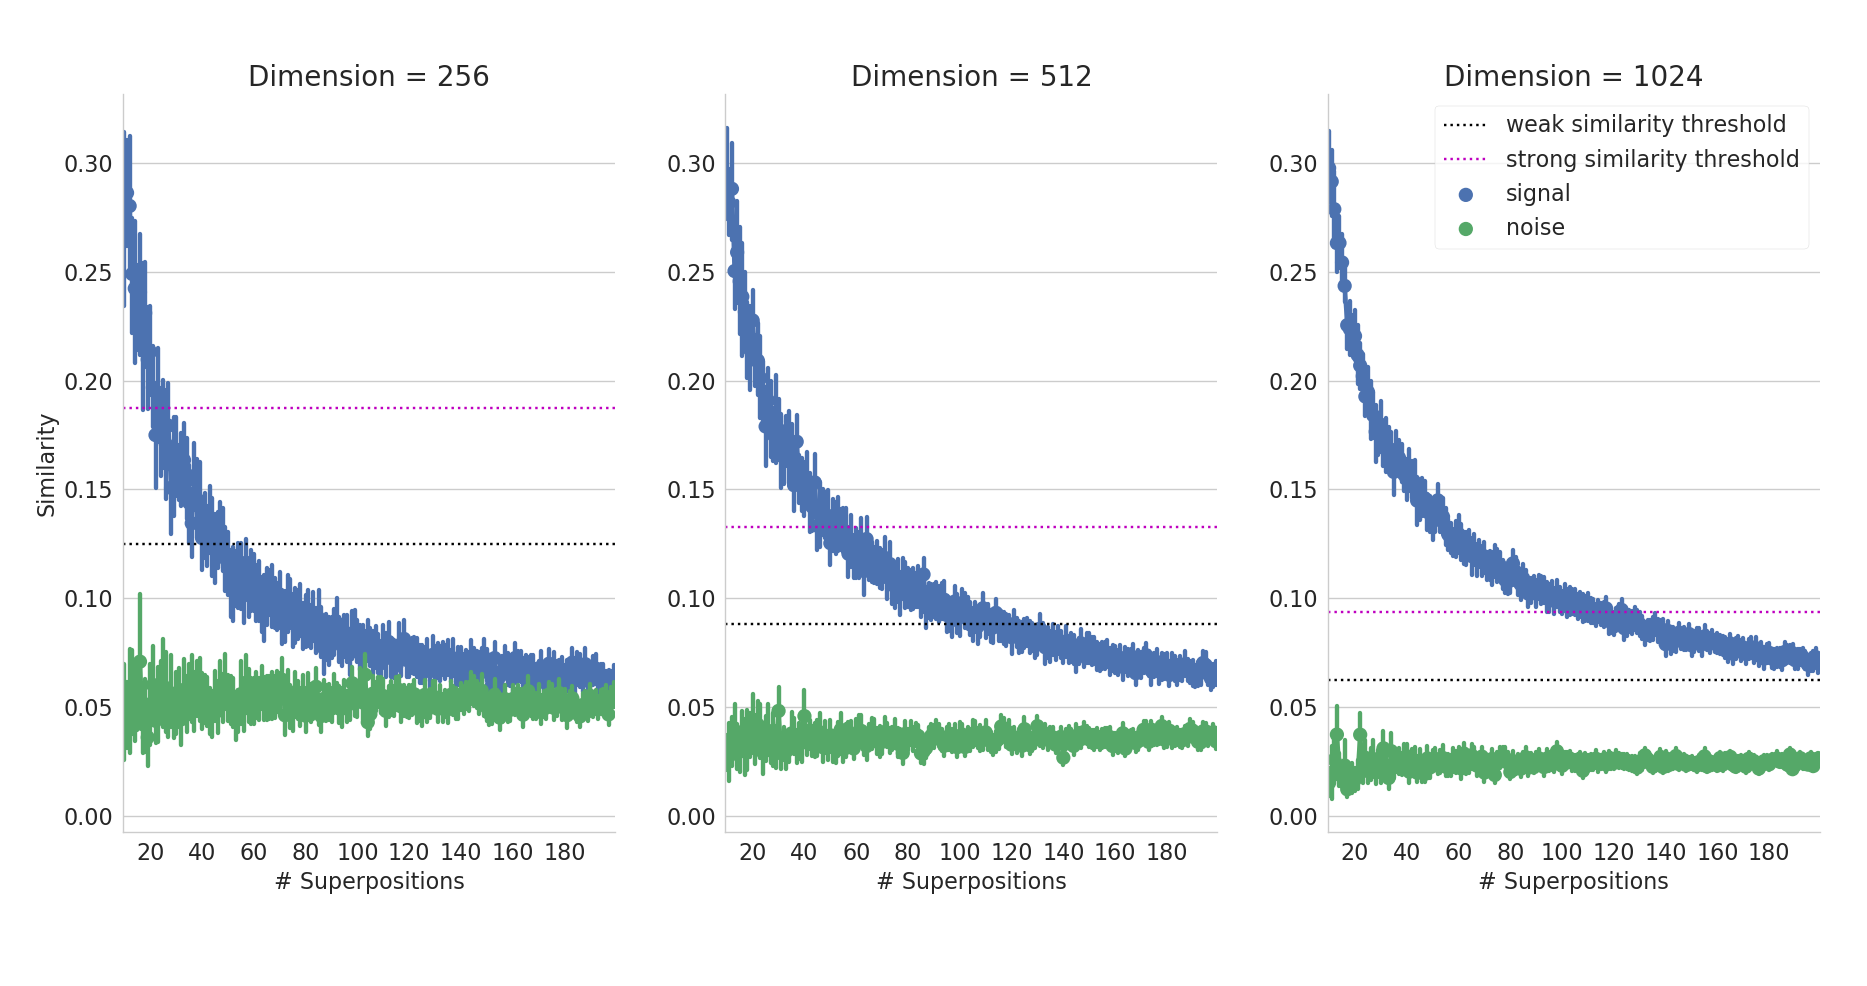
\includegraphics[width=0.95\textwidth]{imgs/spa_superposition_capacity.png}
	\caption{Superposition capacity.}
	\label{fig:spa_superposition_capacity}
\end{figure}